\documentclass{article}
\usepackage{polski}
\usepackage[utf8]{inputenc}
\usepackage{graphicx}
\usepackage{float}

\title{Problem pudełek}
\author{Ahmed Abdelkarim, Aleksandra Hernik}
\begin{document}
\maketitle

\section{Instrukcja obsługi}
Po uruchomieniu programu widoczne jest poniższe okno:
\begin{figure}[H]
\centering
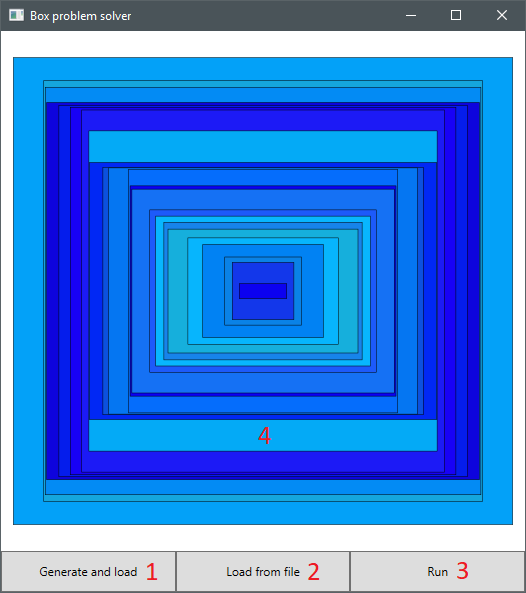
\includegraphics[width=0.8\textwidth]{instrukcja.png}
\caption{Główne okno programu}
\end{figure}
Aby skorzystać z aplikacji, należy najpierw kliknąć na przycisk \textit{Load data} (2) i wybrać plik z danymi wejściowymi. Po zaakceptowaniu pliku pojawi się komunikat o liczbie wczytanych pudełek. \\
Następnie trzeba kliknąć przycisk \textit{Run} (3). W wyniku pojawi się komunikat o długości najdłuższego możliwego ciągu pudełek oraz nazwa pliku wynikowego. Ponadto, w obszarze powyżej guzików (4) zostanie przedstawiona graficzna reprezentacja rozwiązania. Uwaga: wszystkie pudełka są obrócone tak, że dłuższa krawędź to szerokość.  Pudełka są przeskalowane tak, że największe z nich zajmuje całą szerokość okienka. \\
Innym sposobem otrzymania danych wejściowych jest ich wygenerowanie -- w tym celu należy kliknąć na przycisk \textit{Generate and load} (4), aby uzyskać okienko generowania danych, przedstawione poniżej.
\begin{figure}[H]
\centering
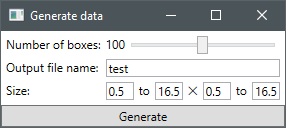
\includegraphics{generate.png}
\caption{Generator danych}
\end{figure}
Pozwala ono wybrać kolejno:
\begin{itemize}
\item Liczbę pudełek (1-200),
\item Nazwę pliku wynikowego,
\item Granice wymiarów pudełek (minimalna i maksymalna szerokość $\times$ minimalna i maksymalna wysokość).
\end{itemize}
Po wciśnięciu przycisku \textit{Generate}, okienko zostanie zamknięte i wygenerowane zostaną pudełka zgodnie z wybranymi opcjami. Jeśli nazwa pliku nie zostanie podana, program wyświetli ostrzeżenie -- dane nie zostaną zapisane, ale będą wczytane do programu. W przypadku niepodania rozszerzenia pliku, automatyczne rozszerzenie to \textit{.txt}.
\clearpage
\section{Opis testów}
\subsection{8 identycznych pudełek}
Dane wejściowe: 8 pudełek, każde o wymiarach 5x10 lub 10x5. \\
Wynik: lista zawierająca jedno pudełko.

\subsection{Duże, 5 średnich, małe}
Dane wejściowe: 7 pudełek, jedno 10x10, jedno 1x1 i pięć 5x5. \\
Wynik: lista zawierająca trzy pudełka: duże, średnie i małe.

\subsection{9 kwadratowych pudełek}
Dane wejściowe: 9 różnych kwadratowych pudełek, o wymiarach od 1x1 do 9x9 (podanych w losowej kolejności).  \\
Wynik: Lista zawierająca wszystkie pudełka.
\begin{figure}[H]
\centering
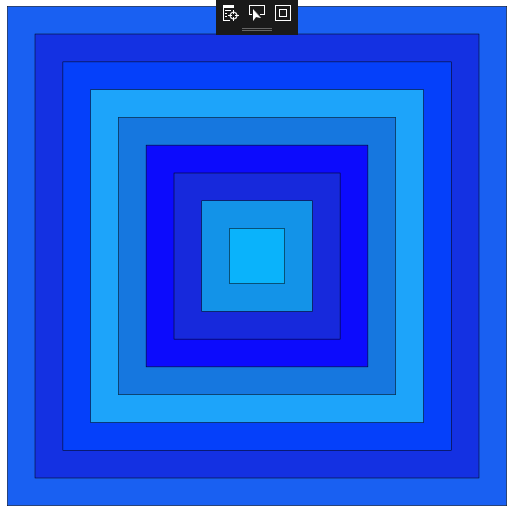
\includegraphics[width=0.8\textwidth]{square_boxes_res.png}
\caption{Graficzna reprezentacja wyniku}
\end{figure}

\subsection{Dwie ścieżki}
Dane wejściowe: 5 pudełek o wymiarach: 11x10, 10x5, 8x6, 7x5, 3x2. W danych istnieją 2 pudełka (8x6 i 10x5), które mieszczą się w większym pudełku, ale nie w sobie nawzajem. Patrząc na pozostałe pudełka można zauważyć, że korzystniejszy jest wybór pudełka o mniejszej powierzchni - 8x6.\\
Wynik: Aplikacja poprawnie dokonuje wyboru uzyskując w ten sposób ciąg 4-elementowy, zamiast 3-elementowy, jak w przypadku, gdyby zostało wybrane złe pudełko.

\subsection{Liczby niecałkowite w danych}
Dane wejściowe: 3 pudełka o wymiarach: 10.01x7.01, 7x10, 6.99x9.99.\\
Wynik: lista składająca się ze wszystkich pudełek. Oznacza to, że liczby wymierne (a nie tylko całkowite) są wczytywane poprawnie.

\subsection{Pudełka nie mieszczące się w sobie nawzajem}
Dane wejściowe: 5 pudełek o wymiarach: 9x1, 8x2, 7x3, 6x4, 5x5. Można zauważyć, że dla każdego pudełka nie istnieje inne, które by się w nim mieściło.\\
Wynik: 1 pudełko. Jako że w zadaniu nie było sprecyzowane zachowanie algorytmu w przypadku kilku poprawnych rozwiązań, zwracane jest tylko jedno z nich (w tym wypadku 9x1).

\subsection{Wylosowane dane - 200 pudełek}
Dane wejściowe: 200 pudełek o wymiarach wylosowanych z przedziału (0.5, 16.5). \\
Wynik: lista 34 pudełek. W tym teście trudno zweryfikować poprawność rozwiązania. Jednak przy założeniu, że rozwiązanie jest poprawne, można wyciągnąć pewne wnioski. Po pierwsze dla 200 pudełek algorytm wykonuje się bardzo szybko. Po drugie po kilku uruchomieniach programu z losowymi danymi dla liczby pudełek równej 200 wynik za każdym razem był z przedziału [30, 40]. Można przypuszczać, że prawdopodobieństwo wystąpienia danych, w których większość pudełek znajdzie się w rozwiązaniu lub w których liczba pudełek w rozwiązaniu będzie bliska 1 jest niewielkie.
\clearpage
\section{Analiza}
Przeprowadzone zostały testy z losowo wygenerowanymi problemami o rozmiarach $1, 11, ... , 991$, dla każdego rozmiaru wartość to średnia z 10 powtórzeń.
\subsection{Czas obliczeń}
Poniższy wykres przedstawia czas działania algorytmu oraz krzywą dopasowaną za pomocą modelu regresji liniowej (zależność $czas ~ n + n^2$). Otrzymane współczynniki to -7.168097e-05 przy $n$ i 3.250486e-07 przy $n^2$.
\begin{figure}[H]
\centering
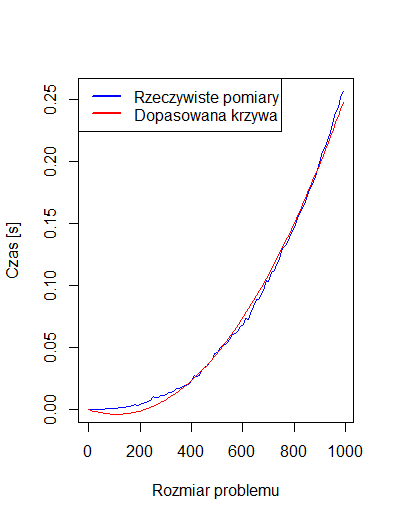
\includegraphics{czasy.png}
\caption{Czas obliczeń}
\end{figure}
Jak widać, otrzymana krzywa jest dobrze dopasowana do pomiarów, co potwierdza wcześniejszą tezę, że algorytm ma złożoność rzędu $O(n^2)$.
\subsection{Frakcja pudełek w najdłuższym ciągu}
W taki sam sposób, jak w przypadku testów czasu obliczeń, została również sprawdzona frakcja pudełek, które znalazły się w znalezionym najdłuższym ciągu. Zgodnie z podejrzeniami, relacja jest malejąca, jak na poniższym wykresie.
\begin{figure}[H]
\centering
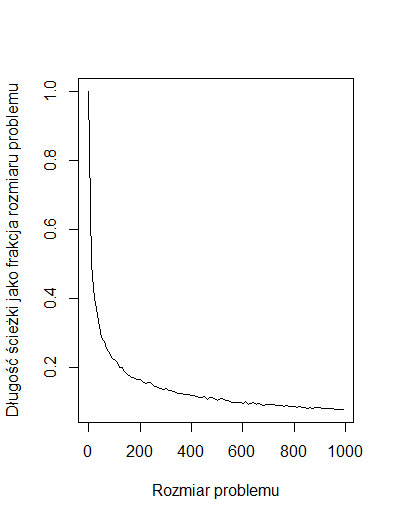
\includegraphics{dlugosc.png}
\caption{Frakcja rozwiązań w wyniku}
\end{figure}
Kształt wykresu przypomina hiperbolę.
\clearpage
\section{Wnioski}
\begin{itemize}
\item Podejście zachłanne (branie zawsze pudełka o największej powierzchni, które zmieści się w ostatnio dodanym pudełku) nie zawsze się sprawdza, co można było zaobserwować w teście 4. Analogiczny problem mógłby napotkać algorytm biorący zawsze najmniejsze pudełko. Jednak algorytm opierający się na przekształceniu problemu na problem grafowy radzi sobie z takimi sytuacjami.
\item Nie jest możliwe określenie rozmiaru wyniku tylko na podstawie rozmiaru wejścia. Dla każdego n istnieje taki problem tego rozmiaru, że wynik zawiera jedno pudełko (test 6) i n pudełek (test 3). Z eksperymentów z losowymi danymi wynika, że dla większych zestawów danych rozmiar rozwiązania nie przekracza 20\% wartości n. Średnia wielkość rozwiązania jako frakcja rozmiaru rozwiązania, w zależności od rozmiaru rozwiązania, jest funkcją malejącą.
\item Istnieją instancje problemów, dla których więcej niż jedno rozwiązanie jest prawdziwe. Niewielka modyfikacja algorytmu (nie zwiększająca złożoności) pozwalałaby na uzyskiwanie wszystkich poprawnych odpowiedzi.
\item Algorytm został zaimplementowany przy założeniu, że pudełko nie mieści się w innym o takich samych wymiarach. Jednak w przypadku rzeczywistych zastosowań nie jest to istotne założenie - jeżeli pudełka są zmierzone dokładnie (na przykład do drugiego miejsca po przecinku) jest mało prawdopodobne, żeby dwa miały dokładnie takie same wymiary, a implementacja dopuszcza wymiary niecałkowite. 
\end{itemize}

\section{Zmiany w stosunku do dokumentacji wstępnej}
\begin{itemize}
\item Na początku wynikowego pliku dodana jest informacja o długości otrzymanej ścieżki.
\item Dla pliku wejściowego o nazwie \textit{file.ext}, plik wyjściowy nazywa się \textit{file\textunderscore output.txt}.
\item Dodany został generator danych.
\end{itemize}

\section{Podział pracy}
Ahmed Abdelkarim zaimplementował interfejs użytkownika, generator danych i algorytm sortowania topologicznego, a Aleksandra Hernik napisała klasy użytkowe (takie jak klasa opisująca graf) i implementację algorytmu znajdowania najdłuższej ścieżki.

\section{Załączniki}
Pliki wejściowe, zawierające zestawy testowe:
\begin{enumerate}
\item \textit{identical\textunderscore boxes.txt} - 8 identycznych pudełek,
\item \textit{big\textunderscore 5medium\textunderscore small.txt} - duże, 5 średnich, małe,
\item \textit{square\textunderscore boxes.txt} - 9 kwadratowych pudełek,
\item \textit{two\textunderscore paths.txt} - dwie ścieżki,
\item \textit{floats.txt} - liczby niecałkowite w danych,
\item \textit{disconnected\textunderscore boxes.txt} - pudełka nie mieszczące się w sobie nawzajem,
\item \textit{random.txt} - wylosowane dane - 200 pudełek.

\end{enumerate}

\end{document}